\documentclass[12pt]{article}
\usepackage[margin=2.5cm]{geometry}
\usepackage{enumerate}
\usepackage{amsfonts}
\usepackage{amsmath}
\usepackage{fancyhdr}
\usepackage{amsmath}
\usepackage{amssymb}
\usepackage{amsthm}
\usepackage{mdframed}
\usepackage{graphicx}
\usepackage{subcaption}
\usepackage{adjustbox}
\usepackage{listings}
\usepackage{xcolor}
\usepackage{booktabs}
\usepackage[utf]{kotex}
\usepackage{hyperref}

\definecolor{codegreen}{rgb}{0,0.6,0}
\definecolor{codegray}{rgb}{0.5,0.5,0.5}
\definecolor{codepurple}{rgb}{0.58,0,0.82}
\definecolor{backcolour}{rgb}{0.95,0.95,0.92}

\lstdefinestyle{mystyle}{
    backgroundcolor=\color{backcolour},
    commentstyle=\color{codegreen},
    keywordstyle=\color{magenta},
    numberstyle=\tiny\color{codegray},
    stringstyle=\color{codepurple},
    basicstyle=\ttfamily\footnotesize,
    breakatwhitespace=false,
    breaklines=true,
    captionpos=b,
    keepspaces=true,
    numbers=left,
    numbersep=5pt,
    showspaces=false,
    showstringspaces=false,
    showtabs=false,
    tabsize=1
}

\lstset{style=mystyle}

\pagestyle{fancy}
\renewcommand{\headrulewidth}{0.4pt}
\lhead{CSC 209}
\rhead{Review 9 Solution}

\begin{document}
\title{CSC 209 Review 9 Solution}
\maketitle

\bigskip

\begin{enumerate}[1.]
    \item

    \begin{enumerate}[a)]
        \item 0

        \bigskip

        \underline{\textbf{Notes}}

        \begin{itemize}
            \item \texttt{a)} is 0 because  (\texttt{i $>>$ 1 + j $>>$ 1 $=$ i $>>$ 10 $>>$ 1 = 0})
            \item
            \textbf{Bitwise Shift Operators}

            \begin{itemize}
                \item has lower precedence than arithematic operators

                \bigskip

                \underline{\textbf{Example:}}

                \bigskip

                \texttt{i $<<$ 2 + 1} means \texttt{i $<<$ (2+1)} and not \texttt{(i $<<$ 2) + 1}

                \bigskip


                \item $<<$ : Left Shift
                \item $>>$ : Right Shift
                \item \textit{Tip:} Always shift only on \underline{unsigned} numbers for portability


                \bigskip

                \underline{\textbf{Example}}

                \bigskip

                \begin{center}
                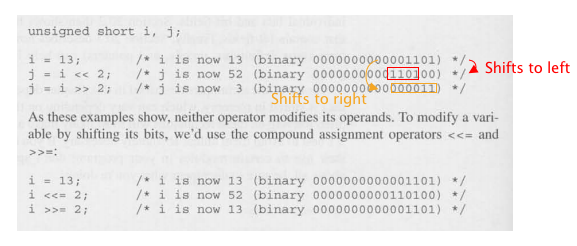
\includegraphics[width=0.9\linewidth]{images/review_9_solution_1.png}
                \end{center}

                \item \texttt{$>>=$} / \texttt{$<<=$} : Are bitwise shift equivalent of \texttt{$+=$}
            \end{itemize}


        \end{itemize}

        \item 0

        \bigskip

        \underline{\textbf{Notes}}

        \begin{itemize}
            \item \texttt{~i} is \texttt{1111111111111111}
            \item \texttt{i} is \texttt{0000000000000000}
            \item so \texttt{~i \& i $=$ 0}
            \item \texttt{~}: Bitwise complement (NOT)

            \bigskip

            \begin{center}
                \begin{tabular}{|c|c|c|}
                    \hline
                    a & $\sim$ a\\
                    \hline
                    0 & 1\\
                    1 & 0\\
                    \hline
                \end{tabular}
            \end{center}

            \bigskip

            \textbf{Example:}

            \bigskip

\begin{lstlisting}[language=c]
    0   1   1   1   //<- this is 7
    --------------
    1   0   0   0   //<- this is 8

    so, ~ 7 = 8
\end{lstlisting}


            \bigskip
            \item \texttt{\&}: Bitwise \textit{and}

            \bigskip

            \begin{center}
                \begin{tabular}{|c|c|c|}
                    \hline
                    a & b & a \& b\\
                    \hline
                    0 & 0  & 0 \\
                    0 & 1  & 1 \\
                    1 & 0  & 0 \\
                    1 & 1  & 1 \\
                    \hline
                \end{tabular}
            \end{center}

            \bigskip

            \textbf{Example:}

            \bigskip

\begin{lstlisting}[language=c]
    0   1   1   1   //<- this is 7
    0   1   0   0   //<- this is 4
    --------------
    0   1   0   0   //<- this is 4

    so, 7 & 4 = 4
\end{lstlisting}

            \bigskip
            \item \texttt{\textrm}: Bitwise \textit{exclusive or}
            \item \texttt{$\vert$}: Bitwise \textit{inclusive or}
        \end{itemize}

        \item 1

        \bigskip

        \underline{\textbf{Notes}}

        \begin{itemize}
            \item \texttt{~i} is \texttt{1111111111111110}
            \item \texttt{j} is \texttt{0000000000000000}
            \item \texttt{~i \& j} is \texttt{0000000000000000} or 1
            \item \texttt{~i \& j \^{} k} is 1
            \item \texttt{\^{}}: Bitwise XOR

            \bigskip

            \begin{center}
                \begin{tabular}{|c|c|c|}
                    \hline
                    a & b & a \^{} b\\
                    \hline
                    0 & 0  & 0 \\
                    0 & 1  & 1 \\
                    1 & 0  & 1 \\
                    1 & 1  & 0 \\
                    \hline
                \end{tabular}
            \end{center}

            \bigskip

            \textbf{Example:}

            \bigskip

    \begin{lstlisting}[language=c]
    0   1   1   1   //<- this is 7
    0   1   0   0   //<- this is 4
    --------------
    0   0   1   1   //<- this is 3

    so, 7 ^ 4 = 3
    \end{lstlisting}
        \end{itemize}

        \item 0

        \bigskip

        \underline{\textbf{Example}}

        \begin{itemize}
            \item \texttt{i} is \texttt{0000000000000111}
            \item \texttt{j} is \texttt{0000000000001000}
            \item \texttt{i \^{} j} is \texttt{0000000000000000} or 0
            \item \texttt{k} is \texttt{0000000000001001}
            \item \texttt{i \^{} j \& k} is \texttt{0000000000000000} or 0
        \end{itemize}

        \bigskip

        \begin{mdframed}
        \underline{\textbf{Correct Solution}}

        \bigskip

        \color{red}15\color{black}
        \end{mdframed}

        \bigskip

        \underline{\textbf{Notes}}

        \begin{itemize}
            \item There is a precendence to the order of operations

            \begin{center}
            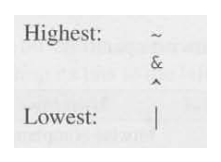
\includegraphics[width=0.4\linewidth]{images/review_9_solution_2.png}
            \end{center}
        \end{itemize}

        \item

        \begin{itemize}
            \item toggling from 0 to 1

            \bigskip

            \texttt{i = 0x0000;}

            \texttt{i $\lvert$= 0x0001;}

            \bigskip

            or

            \bigskip

            \texttt{i $\lvert$= 1 $<<$ 0;} where \texttt{i = 0x0000;}

            \item toggling from 1 to 0

            \bigskip

            \texttt{i = 0x0001;}

            \texttt{i $\&$= $\sim$0x0001;}

            \bigskip

            or

            \bigskip

            \texttt{i $\&$= $\sim$(1 $<<$ 0);} where \texttt{i = 0x0001;}
        \end{itemize}

        \bigskip

        \begin{mdframed}
        \underline{\textbf{Correct Solution}}

        \begin{itemize}
            \item toggling from 0 to 1 of \color{red}4th bit\color{black}

            \bigskip

            \color{red}\texttt{i = 0x0010;}\color{black}

            \texttt{i \^{}= 0x0000;}

            \bigskip

            or

            \bigskip

            \texttt{i \^{}= 1 $<<$ 4;} where \texttt{i = 0x0000;}

            \item toggling from 1 to 0 of \color{red}4th bit\color{black}

            \bigskip

            \texttt{i = 0x0010;}

            \texttt{i \^{}= 0x0010;}

            \bigskip

            or

            \bigskip

            \texttt{i \^{}= (1 $<<$ 4);} where \texttt{i = 0x0010;}
        \end{itemize}

        \end{mdframed}

        \bigskip

        \underline{\textbf{Notes}}

        \begin{itemize}
            \item Toggling can be done using bitwise XOR


            \item \textbf{Setting a bit}

            \begin{itemize}
                \item Is done using $\vert$ or bitwise OR

                \begin{center}
                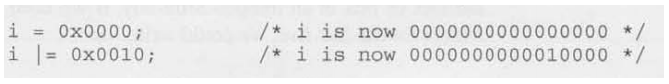
\includegraphics[width=\linewidth]{images/review_9_solution_3.png}
                \end{center}

                \item The idiom of above is \texttt{i $\lvert=$ 1 $<<$ j}
            \end{itemize}

            \item \textbf{Clearing a bit}

            \begin{itemize}
                \item Is done using $\vert$ or bitwise AND

                \begin{center}
                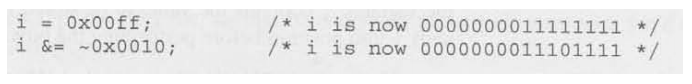
\includegraphics[width=\linewidth]{images/review_9_solution_5.png}
                \end{center}

                \item The idiom of above is \texttt{i \&= $\sim$(i $<<$ j)}
            \end{itemize}
        \end{itemize}

    \end{enumerate}

    \item It swaps the elements between \texttt{x} and \texttt{y}.

    \underline{\textbf{Notes}}

    \begin{itemize}
        \item Preprocessor performs operations of statements in order from left to right

        \begin{center}
        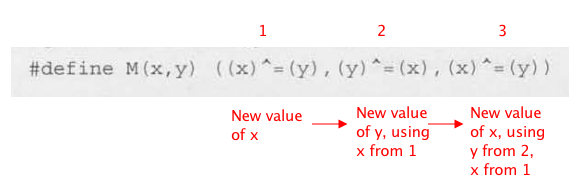
\includegraphics[width=\linewidth]{images/review_9_solution_6.png}
        \end{center}
    \end{itemize}

    \item

    \texttt{\#define MK\_COLOR(r,g,b) (long) ( (b | (g $<<$ 8)) | (b | (r $<<$ 16)))}

    \bigskip

    \underline{\textbf{Rough Work}}

    \begin{enumerate}[1.]

        \item store \texttt{b} in bit 0

        \bigskip

        \texttt{b}

        \bigskip

        \item store \texttt{g} in bit 8

        \bigskip

        \texttt{b $\lvert$ g $<<$ 8}

        \bigskip

        \item store \texttt{r} in bit 16

        \texttt{ b $\lvert$  r $<<$ 16}

        \bigskip
    \end{enumerate}

    \bigskip

    \begin{mdframed}
    \underline{\textbf{Correct Solution}}

    \bigskip

    \texttt{\#define MK\_COLOR(r,g,b) (long) ((\color{red}r\color{black} | (g $<<$ 8)) | (\color{red}r\color{black} | (\color{red}b\color{black} $<<$ 16)))\color{black}}
    \end{mdframed}

    \underline{\textbf{Notes}}

    \begin{itemize}
        \item First Byte is furthest from \texttt{0x} and first byte is closest to \texttt{0x}

        \bigskip

        \begin{center}
        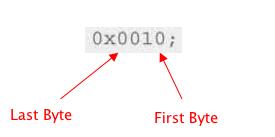
\includegraphics[width=0.6\linewidth]{images/review_9_solution_7.png}
        \end{center}
    \end{itemize}

    \item

    \begin{itemize}
        \item \texttt{GET\_RED}

        \bigskip

        \texttt{\#define GET\_RED(c) (long) (c \& 0x007)}

        \bigskip

        \item \texttt{GET\_GREEN}

        \bigskip

        \texttt{\#define GET\_GREEN(c) (long) ((c $>>$ 8) \& 0x007)}

        \bigskip

        \item \texttt{GET\_BLUE}

        \bigskip

        \texttt{\#define GET\_BLUE(c) (long) ((c $>>$ 16) \& 0x007)}

        \bigskip
    \end{itemize}

    \bigskip

    \underline{\textbf{Notes}}

    \begin{itemize}
        \item \texttt{0x0007} in binary is \texttt{0x0000000000001111}
        \item \texttt{c $>>$ 4} shifts \texttt{c} to right by 4 bits and return
        overlapping value between {c $>>$ 4} and \texttt{0x0000000000001111} (\texttt{0x007})
        \item Test code is below

\begin{lstlisting}[language=c]
    #include <stdio.h>
    #include <stdlib.h>

    #define MK_COLOR(r,g,b) (long) ( (r | (g << 8)) | (r | (b << 16)))
    #define GET_RED(c) (long) (c & 0x007)
    #define GET_GREEN(c) (long) ((c >> 8) & 0x007)
    #define GET_BLUE(c) (long) ((c >> 16) & 0x007)

    int main() {
        long i, r = 4, g = 5, b = 6, r2, g2, b2;

        i = MK_COLOR(r,g,b);

        r2 = GET_RED(i);
        g2 = GET_GREEN(i);
        b2 = GET_BLUE(i);

        printf("%ld\n", i);
        printf("%ld\n", r2);
        printf("%ld\n", g2);
        printf("%ld\n", b2);

        return 0;
    }
\end{lstlisting}
    \end{itemize}

    \item

    \begin{enumerate}[a)]

        \item

\begin{lstlisting}[language=c]
    unsigned short swap_bytes(unsigned short i) {
        unsigned short j, k;

        j = i & 0x007; // extract first byte

        i = i >> 4;
        k = i & 0x007; // extract second byte

        i = i >> 4; // shift down layter two bytes

        i |= j << 8; // add first byte to position of fourth byte
        i |= k << 12; // add second byte to position of third byte

    }
\end{lstlisting}

        \item

\begin{lstlisting}[language=c]
    unsigned short swap_bytes(unsigned short i) {

        i = i >> 8 | i << 8;

        return i;
    }
\end{lstlisting}

    \end{enumerate}

    \bigskip

    \underline{\textbf{Rough Works}}

    \bigskip

    \begin{enumerate}[1.]
        \item Extract first two bytes

        \bigskip

        \texttt{j = i \& 0x0007}

        \texttt{i = i $>>$ 4}

        \texttt{k = i \& 0x0007}

        \bigskip

        \item Shift later two bytes down

        \bigskip

        \texttt{i = i $>>$ 4}

        \bigskip

        \item Add first two bytes to last two bytes

        \bigskip

        \texttt{i |= j $<<$ 8};

        \texttt{i |= k $<<$ 12};

        \bigskip

    \end{enumerate}

    \item

\begin{lstlisting}[language=c]
    unsigned int rotate_left(unsigned int i, int n) {
        return i >> 28 | i << n;
    }

    unsigned int rotate_right(unsigned int i, int n) {
        return i << 28 | i >> n;
    }
\end{lstlisting}

    \item

    \begin{enumerate}[a)]
        \item Is a binary with \texttt{n} many 1s from the first bit
        \item Extracts last \texttt{n} bits in \texttt{i}
    \end{enumerate}

    \bigskip

    \begin{mdframed}

    \underline{\textbf{Correct Solution}}

    \bigskip

    \begin{enumerate}[a)]
        \item Is a binary with \texttt{n} many 1s from the first bit
        \item Extracts last \texttt{n} bits \color{red}starting from position \texttt{m}\color{black}\:in \texttt{i}
    \end{enumerate}

    \end{mdframed}

    \item

    \begin{enumerate}[a)]
        \item

\begin{lstlisting}[language=c]
    unsigned int count_ones(unsigned char *ch)
    {
        unsigned char *p;
        unsigned int count;

        for (p = ch; *p != '\0'; p++){
            if (*p == '1') {
                count++;
            }
        }

        return count;
    }
\end{lstlisting}

        \item

\begin{lstlisting}[language=c]
    unsigned int count_ones(unsigned char ch)
    {
        int sum = 0;

        sum += (i >> 0) & 1;
        sum += (i >> 1) & 1;
        sum += (i >> 2) & 1;
        sum += (i >> 3) & 1;
        sum += (i >> 4) & 1;
        sum += (i >> 5) & 1;
        sum += (i >> 6) & 1;
        sum += (i >> 7) & 1;
        return count;
    }
\end{lstlisting}

        \bigskip

        \underline{\textbf{Notes}}

        \begin{itemize}
            \item Unsigned char goes from 0 (00000000) to 255 (11111111)
            \item I am having trouble how to convert from loop to with out loop :'(.
            I need help
            \item Example

            \bigskip

            100010101 - Here there are 4 1s.

            \bigskip
        \end{itemize}

    \end{enumerate}


\end{enumerate}

\end{document}